% *********************************************************************
% © 2010–2022 Jeremy Sylvestre
%
% Permission is granted to copy, distribute and/or modify this document
% under the terms of the GNU Free Documentation License, Version 1.3 or
% any later version published by the Free Software Foundation; with no
% Invariant Sections, no Front-Cover Texts, and no Back-Cover Texts. A
% copy of the license is included in the appendix entitled “GNU Free
% Documentation License” that appears in the output document of this
% PreTeXt source code. All trademarks™ are the registered® marks of
% their respective owners.
%
% *********************************************************************

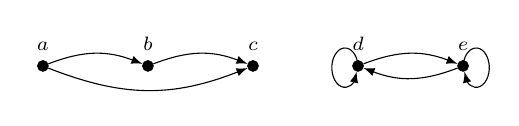
\begin{tikzpicture}[
	xscale=0.667,
	vertex/.style={ circle, draw, very thin, fill, inner sep=0pt, minimum size=4pt },
	vertexg/.style={ black!40!white, circle, draw, very thin, fill, inner sep=0pt, minimum size=4pt },
	vertexo/.style={ circle, draw, very thin, inner sep=0pt, minimum size=4pt }
]

\node at (0,0) (a) [vertex,label=above:$\scriptstyle a$] {};
\node at (2,0) (b) [vertex,label=above:$\scriptstyle b$] {};
\node at (4,0) (c) [vertex,label=above:$\scriptstyle c$] {};
\node at (6,0) (d) [vertex,label=above:$\scriptstyle d$] {};
\node at (8,0) (e) [vertex,label=above:$\scriptstyle e$] {};
\draw[-latex] (a) to [out=15,in=165] (b);
\draw[-latex] (b) to [out=15,in=165] (c);
\draw[-latex] (a) to [out=-15,in=-165] (c);
\draw[-latex] (d) to [out=15,in=165] (e);
\draw[-latex] (e) to [out=195,in=-15] (d);
\draw[-latex] (d) arc (5:315:0.25cm) to (d);
\draw[-latex] (e) arc (175:-135:0.25cm) to (e);

\end{tikzpicture}
